\documentclass[12pt, twoside]{article}
\usepackage[francais]{babel}
\usepackage[T1]{fontenc}
\usepackage[latin1]{inputenc}
\usepackage[left=6mm, right=6mm, top=6mm, bottom=6mm]{geometry}
\usepackage{float}
\usepackage{graphicx}
\usepackage{array}
\usepackage{multirow}
\usepackage{amsmath,amssymb,mathrsfs}
\usepackage{textcomp}
\usepackage{soul}

\pagestyle{empty}
\begin{document}


\begin{flushleft}
Nom : \\
Prenom : 
\end{flushleft}

\begin{center}
{\fbox{$6^{e}D$ \qquad \qquad \textbf{\Large{Contr�le}}
\qquad \qquad 11/12/2008}}
\end{center}


\textit{Les exercices 1,2 et 3 sont � faire sur les photocopies.}
\bigskip

\textbf{Exercice 1:}

\begin{center}
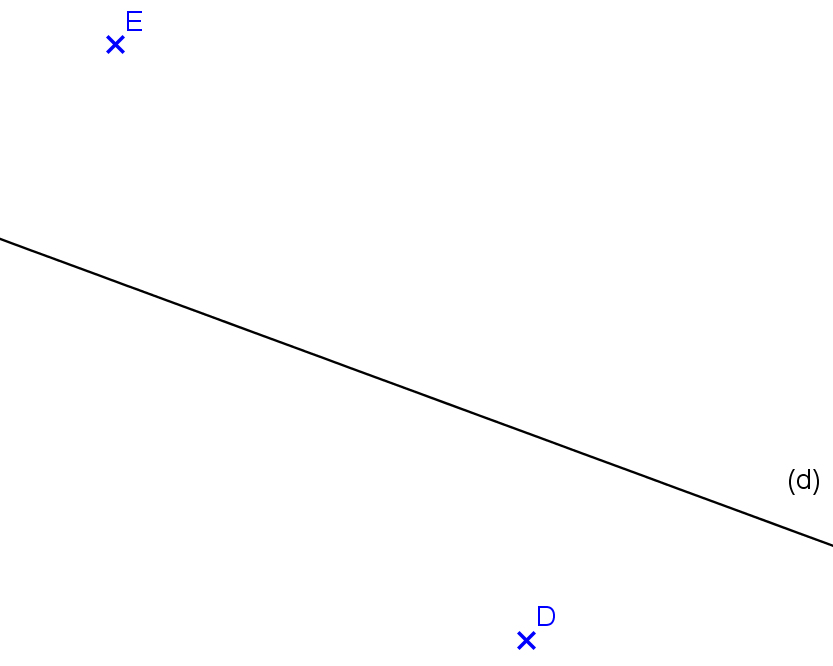
\includegraphics[width=7cm]{images/ex1.png} 
\end{center}

\begin{enumerate}
  \item Tracer en rouge la droite $(d_{1})$ perpendiculaire � $(d)$ passant par
  $D$.
  \item Tracer en vert la droite $(d_{2})$ perpendiculaire � $(d)$ passant par
  $E$.
  \item Que peut-on dire des doites $(d_{1})$ et $(d_{2})$?
 
 \rule{180mm}{0.5pt}
 
 
 \rule{180mm}{0.5pt}
 \item Citer la propri�t� du cours qui permet de l'affirmer?
  
  \rule{180mm}{0.5pt}
  
  \rule{180mm}{0.5pt}
  
  \rule{180mm}{0.5pt}
  
  \rule{180mm}{0.5pt}
  \item  Compl�ter:
 \begin{center}
 
\begin{tabular}{cc}
 \begin{minipage}{6cm}
 \ul{Donn�es}\\
 \ldots \ldots \ldots \ldots \ldots\\
 \ldots \ldots \ldots \ldots \ldots
 \end{minipage}       
&  
\begin{minipage}{6cm}
\ul{Conclusion}
\medskip

donc \ldots \ldots \ldots \ldots
\end{minipage}
 \end{tabular}
  \end{center}
  \end{enumerate}
 
\bigskip  
\bigskip

\textbf{Exercice 2:}


\begin{center} 
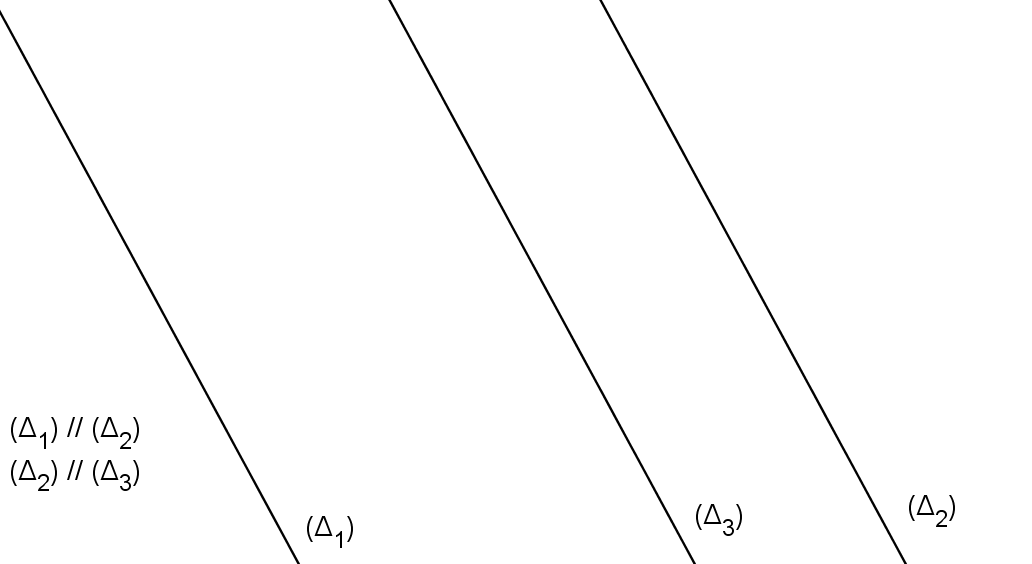
\includegraphics[width=8cm]{images/ex2.png} 
\end{center} 



\begin{enumerate}
 \item Que peut-on dire des doites $(\Delta_{1})$ et $(\Delta_{3})$?
 
 \rule{180mm}{0.5pt}
 
 
 \rule{180mm}{0.5pt}
\begin{flushleft}
Nom : \\
Prenom : 
\end{flushleft}
 \item Citer la propri�t� du cours qui permet de l'affirmer?
   
  \rule{180mm}{0.5pt}
  
  \rule{180mm}{0.5pt}
  
  \rule{180mm}{0.5pt}
  
  \rule{180mm}{0.5pt}
  \item  Compl�ter:
 \begin{center}
 
\begin{tabular}{cc}
 \begin{minipage}{6cm}
 \ul{Donn�es}\\
 \ldots \ldots \ldots \ldots \ldots\\
 \ldots \ldots \ldots \ldots \ldots
 \end{minipage}       
&  
\begin{minipage}{6cm}
\ul{Conclusion}
\medskip

donc \ldots \ldots \ldots \ldots
\end{minipage}
 \end{tabular}
  \end{center}
  \end{enumerate}
 
\bigskip  
\bigskip 

\textbf{Exercice 3:}
\begin{center}
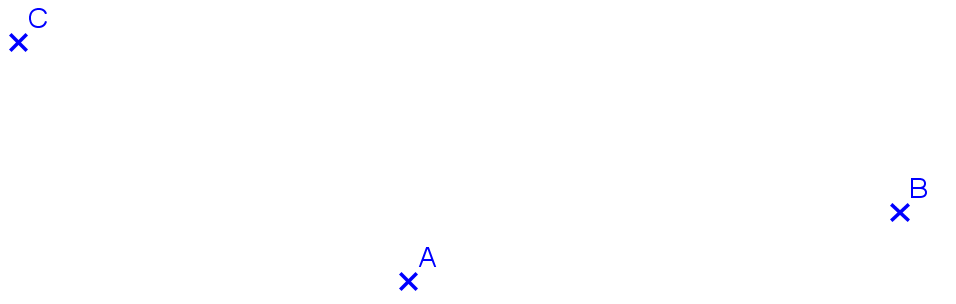
\includegraphics[width=10cm]{images/ex3.png}
\end{center}

\bigskip
\bigskip

\begin{enumerate}
  \item Construire en rouge la droite $(d)$ parall�le � $(AB)$ passant par
  $C$. Ecrire cette phrase en symbole math�matique � c�t� de la
  figure.
  \item Construire en vert la droite $(d_{1})$ perpendiculaire � $(AB)$ passant
  par $C$ et coder la figure.
 \item Que peut-on dire des doites $(d)$ et $(d_{1})$?
 
 \rule{180mm}{0.5pt}
 
 
 \rule{180mm}{0.5pt}
 \item Citer la propri�t� du cours qui permet de l'affirmer?
  
  \rule{180mm}{0.5pt}
  
  \rule{180mm}{0.5pt}
  
  \rule{180mm}{0.5pt}
  
  \rule{180mm}{0.5pt}
  \item  Compl�ter:
 \begin{center}
 
\begin{tabular}{cc}
 \begin{minipage}{6cm}
 \ul{Donn�es}\\
 \ldots \ldots \ldots \ldots \ldots\\
 \ldots \ldots \ldots \ldots \ldots
 \end{minipage}       
&  
\begin{minipage}{6cm}
\ul{Conclusion}
\medskip

donc \ldots \ldots \ldots \ldots
\end{minipage}
 \end{tabular}
  \end{center}
  \end{enumerate}
 
\bigskip  
\bigskip 


\textbf{Exercice 4:} 

\bigskip

\begin{tabular}{cc}
\begin{minipage}{8cm}
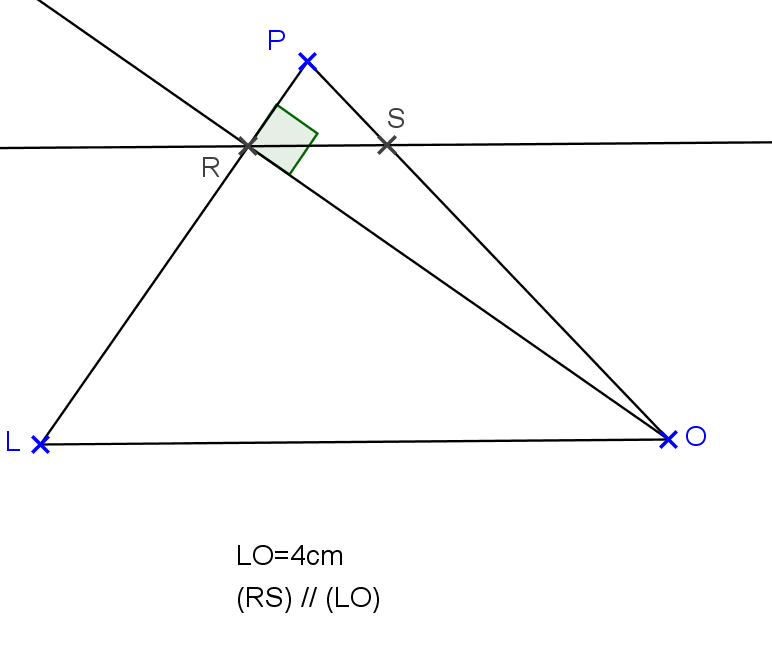
\includegraphics[width=6cm]{images/ex4.png}
\end{minipage}
&
\begin{minipage}{10cm}
Arthur doit construire la figure de gauche. Il a pour le moment la figure
suivante: 


\includegraphics[width=3cm]{images/ex5.png}

Quelles consignes doit-on lui donner pour qu'il compl�te son dessin et obtienne
la figure demand�e? Les �crire sur votre copie.
\end{minipage}
\end{tabular}

\medskip
\textit{Remarque: on ne demande pas de faire la figure.}
\end{document}